% Created by tikzDevice version 0.12.3.1 on 2022-03-10 11:32:19
% !TEX encoding = UTF-8 Unicode
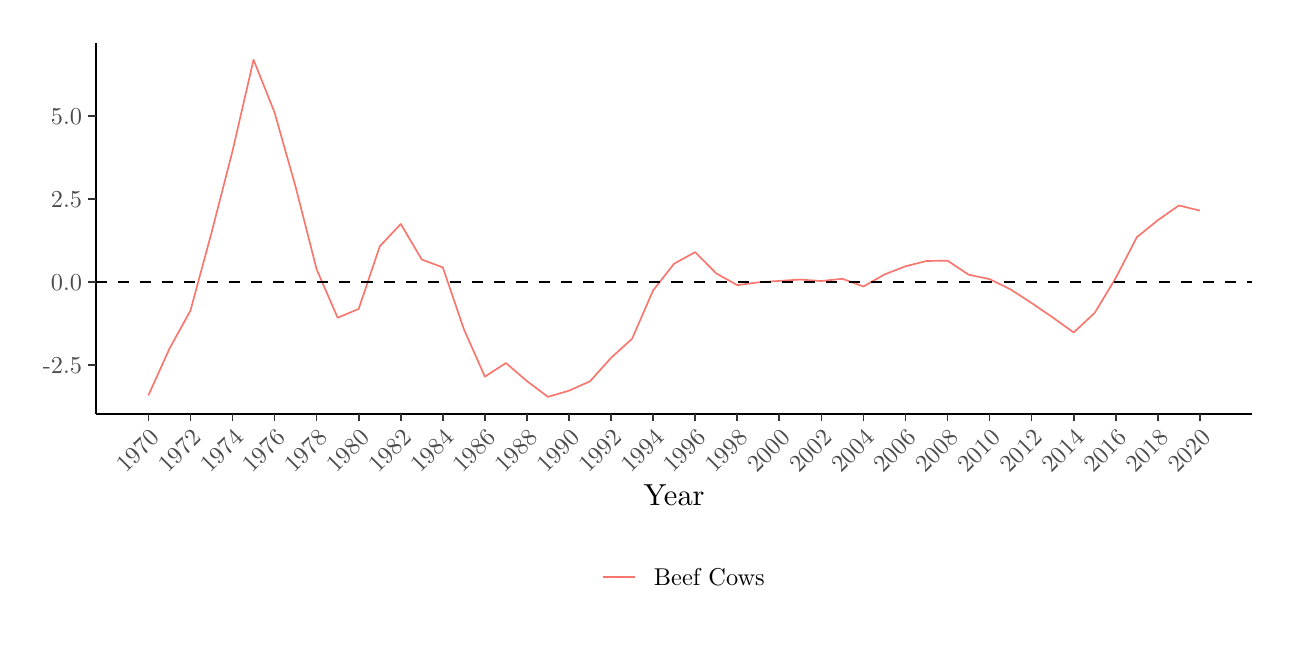
\begin{tikzpicture}[x=1pt,y=1pt]
\definecolor{fillColor}{RGB}{255,255,255}
\path[use as bounding box,fill=fillColor,fill opacity=0.00] (0,0) rectangle (448.07,216.81);
\begin{scope}
\path[clip] (  0.00,  0.00) rectangle (448.07,216.81);
\definecolor{drawColor}{RGB}{255,255,255}
\definecolor{fillColor}{RGB}{255,255,255}

\path[draw=drawColor,line width= 0.6pt,line join=round,line cap=round,fill=fillColor] (  0.00,  0.00) rectangle (448.07,216.81);
\end{scope}
\begin{scope}
\path[clip] ( 24.62, 77.31) rectangle (442.57,211.31);
\definecolor{fillColor}{RGB}{255,255,255}

\path[fill=fillColor] ( 24.62, 77.31) rectangle (442.57,211.31);
\definecolor{drawColor}{RGB}{248,118,109}

\path[draw=drawColor,line width= 0.6pt,line join=round] ( 43.62, 83.93) --
	( 51.22,100.79) --
	( 58.82,114.59) --
	( 66.42,142.66) --
	( 74.02,172.26) --
	( 81.62,205.22) --
	( 89.22,186.13) --
	( 96.82,159.29) --
	(104.41,129.48) --
	(112.01,112.00) --
	(119.61,115.17) --
	(127.21,137.77) --
	(134.81,145.87) --
	(142.41,133.02) --
	(150.01,130.18) --
	(157.61,107.89) --
	(165.21, 90.70) --
	(172.81, 95.63) --
	(180.41, 89.11) --
	(188.00, 83.40) --
	(195.60, 85.63) --
	(203.20, 89.03) --
	(210.80, 97.49) --
	(218.40,104.41) --
	(226.00,121.88) --
	(233.60,131.54) --
	(241.20,135.71) --
	(248.80,128.01) --
	(256.40,123.77) --
	(264.00,124.78) --
	(271.59,125.30) --
	(279.19,125.80) --
	(286.79,125.25) --
	(294.39,126.07) --
	(301.99,123.28) --
	(309.59,127.62) --
	(317.19,130.58) --
	(324.79,132.50) --
	(332.39,132.61) --
	(339.99,127.55) --
	(347.59,125.94) --
	(355.18,122.24) --
	(362.78,117.30) --
	(370.38,112.12) --
	(377.98,106.65) --
	(385.58,113.78) --
	(393.18,126.38) --
	(400.78,141.07) --
	(408.38,147.24) --
	(415.98,152.56) --
	(423.58,150.70);
\definecolor{drawColor}{RGB}{0,0,0}

\path[draw=drawColor,line width= 0.6pt,dash pattern=on 4pt off 4pt ,line join=round] ( 24.62,124.90) -- (442.57,124.90);
\end{scope}
\begin{scope}
\path[clip] (  0.00,  0.00) rectangle (448.07,216.81);
\definecolor{drawColor}{RGB}{0,0,0}

\path[draw=drawColor,line width= 0.6pt,line join=round] ( 24.62, 77.31) --
	( 24.62,211.31);
\end{scope}
\begin{scope}
\path[clip] (  0.00,  0.00) rectangle (448.07,216.81);
\definecolor{drawColor}{gray}{0.30}

\node[text=drawColor,anchor=base east,inner sep=0pt, outer sep=0pt, scale=  0.88] at ( 19.67, 91.89) {-2.5};

\node[text=drawColor,anchor=base east,inner sep=0pt, outer sep=0pt, scale=  0.88] at ( 19.67,121.87) {0.0};

\node[text=drawColor,anchor=base east,inner sep=0pt, outer sep=0pt, scale=  0.88] at ( 19.67,151.84) {2.5};

\node[text=drawColor,anchor=base east,inner sep=0pt, outer sep=0pt, scale=  0.88] at ( 19.67,181.82) {5.0};
\end{scope}
\begin{scope}
\path[clip] (  0.00,  0.00) rectangle (448.07,216.81);
\definecolor{drawColor}{gray}{0.20}

\path[draw=drawColor,line width= 0.6pt,line join=round] ( 21.87, 94.92) --
	( 24.62, 94.92);

\path[draw=drawColor,line width= 0.6pt,line join=round] ( 21.87,124.90) --
	( 24.62,124.90);

\path[draw=drawColor,line width= 0.6pt,line join=round] ( 21.87,154.87) --
	( 24.62,154.87);

\path[draw=drawColor,line width= 0.6pt,line join=round] ( 21.87,184.85) --
	( 24.62,184.85);
\end{scope}
\begin{scope}
\path[clip] (  0.00,  0.00) rectangle (448.07,216.81);
\definecolor{drawColor}{RGB}{0,0,0}

\path[draw=drawColor,line width= 0.6pt,line join=round] ( 24.62, 77.31) --
	(442.57, 77.31);
\end{scope}
\begin{scope}
\path[clip] (  0.00,  0.00) rectangle (448.07,216.81);
\definecolor{drawColor}{gray}{0.20}

\path[draw=drawColor,line width= 0.6pt,line join=round] ( 43.62, 74.56) --
	( 43.62, 77.31);

\path[draw=drawColor,line width= 0.6pt,line join=round] ( 58.82, 74.56) --
	( 58.82, 77.31);

\path[draw=drawColor,line width= 0.6pt,line join=round] ( 74.02, 74.56) --
	( 74.02, 77.31);

\path[draw=drawColor,line width= 0.6pt,line join=round] ( 89.22, 74.56) --
	( 89.22, 77.31);

\path[draw=drawColor,line width= 0.6pt,line join=round] (104.41, 74.56) --
	(104.41, 77.31);

\path[draw=drawColor,line width= 0.6pt,line join=round] (119.61, 74.56) --
	(119.61, 77.31);

\path[draw=drawColor,line width= 0.6pt,line join=round] (134.81, 74.56) --
	(134.81, 77.31);

\path[draw=drawColor,line width= 0.6pt,line join=round] (150.01, 74.56) --
	(150.01, 77.31);

\path[draw=drawColor,line width= 0.6pt,line join=round] (165.21, 74.56) --
	(165.21, 77.31);

\path[draw=drawColor,line width= 0.6pt,line join=round] (180.41, 74.56) --
	(180.41, 77.31);

\path[draw=drawColor,line width= 0.6pt,line join=round] (195.60, 74.56) --
	(195.60, 77.31);

\path[draw=drawColor,line width= 0.6pt,line join=round] (210.80, 74.56) --
	(210.80, 77.31);

\path[draw=drawColor,line width= 0.6pt,line join=round] (226.00, 74.56) --
	(226.00, 77.31);

\path[draw=drawColor,line width= 0.6pt,line join=round] (241.20, 74.56) --
	(241.20, 77.31);

\path[draw=drawColor,line width= 0.6pt,line join=round] (256.40, 74.56) --
	(256.40, 77.31);

\path[draw=drawColor,line width= 0.6pt,line join=round] (271.59, 74.56) --
	(271.59, 77.31);

\path[draw=drawColor,line width= 0.6pt,line join=round] (286.79, 74.56) --
	(286.79, 77.31);

\path[draw=drawColor,line width= 0.6pt,line join=round] (301.99, 74.56) --
	(301.99, 77.31);

\path[draw=drawColor,line width= 0.6pt,line join=round] (317.19, 74.56) --
	(317.19, 77.31);

\path[draw=drawColor,line width= 0.6pt,line join=round] (332.39, 74.56) --
	(332.39, 77.31);

\path[draw=drawColor,line width= 0.6pt,line join=round] (347.59, 74.56) --
	(347.59, 77.31);

\path[draw=drawColor,line width= 0.6pt,line join=round] (362.78, 74.56) --
	(362.78, 77.31);

\path[draw=drawColor,line width= 0.6pt,line join=round] (377.98, 74.56) --
	(377.98, 77.31);

\path[draw=drawColor,line width= 0.6pt,line join=round] (393.18, 74.56) --
	(393.18, 77.31);

\path[draw=drawColor,line width= 0.6pt,line join=round] (408.38, 74.56) --
	(408.38, 77.31);

\path[draw=drawColor,line width= 0.6pt,line join=round] (423.58, 74.56) --
	(423.58, 77.31);
\end{scope}
\begin{scope}
\path[clip] (  0.00,  0.00) rectangle (448.07,216.81);
\definecolor{drawColor}{gray}{0.30}

\node[text=drawColor,rotate= 45.00,anchor=base east,inner sep=0pt, outer sep=0pt, scale=  0.88] at ( 47.91, 68.07) {1970};

\node[text=drawColor,rotate= 45.00,anchor=base east,inner sep=0pt, outer sep=0pt, scale=  0.88] at ( 63.11, 68.07) {1972};

\node[text=drawColor,rotate= 45.00,anchor=base east,inner sep=0pt, outer sep=0pt, scale=  0.88] at ( 78.30, 68.07) {1974};

\node[text=drawColor,rotate= 45.00,anchor=base east,inner sep=0pt, outer sep=0pt, scale=  0.88] at ( 93.50, 68.07) {1976};

\node[text=drawColor,rotate= 45.00,anchor=base east,inner sep=0pt, outer sep=0pt, scale=  0.88] at (108.70, 68.07) {1978};

\node[text=drawColor,rotate= 45.00,anchor=base east,inner sep=0pt, outer sep=0pt, scale=  0.88] at (123.90, 68.07) {1980};

\node[text=drawColor,rotate= 45.00,anchor=base east,inner sep=0pt, outer sep=0pt, scale=  0.88] at (139.10, 68.07) {1982};

\node[text=drawColor,rotate= 45.00,anchor=base east,inner sep=0pt, outer sep=0pt, scale=  0.88] at (154.29, 68.07) {1984};

\node[text=drawColor,rotate= 45.00,anchor=base east,inner sep=0pt, outer sep=0pt, scale=  0.88] at (169.49, 68.07) {1986};

\node[text=drawColor,rotate= 45.00,anchor=base east,inner sep=0pt, outer sep=0pt, scale=  0.88] at (184.69, 68.07) {1988};

\node[text=drawColor,rotate= 45.00,anchor=base east,inner sep=0pt, outer sep=0pt, scale=  0.88] at (199.89, 68.07) {1990};

\node[text=drawColor,rotate= 45.00,anchor=base east,inner sep=0pt, outer sep=0pt, scale=  0.88] at (215.09, 68.07) {1992};

\node[text=drawColor,rotate= 45.00,anchor=base east,inner sep=0pt, outer sep=0pt, scale=  0.88] at (230.29, 68.07) {1994};

\node[text=drawColor,rotate= 45.00,anchor=base east,inner sep=0pt, outer sep=0pt, scale=  0.88] at (245.48, 68.07) {1996};

\node[text=drawColor,rotate= 45.00,anchor=base east,inner sep=0pt, outer sep=0pt, scale=  0.88] at (260.68, 68.07) {1998};

\node[text=drawColor,rotate= 45.00,anchor=base east,inner sep=0pt, outer sep=0pt, scale=  0.88] at (275.88, 68.07) {2000};

\node[text=drawColor,rotate= 45.00,anchor=base east,inner sep=0pt, outer sep=0pt, scale=  0.88] at (291.08, 68.07) {2002};

\node[text=drawColor,rotate= 45.00,anchor=base east,inner sep=0pt, outer sep=0pt, scale=  0.88] at (306.28, 68.07) {2004};

\node[text=drawColor,rotate= 45.00,anchor=base east,inner sep=0pt, outer sep=0pt, scale=  0.88] at (321.47, 68.07) {2006};

\node[text=drawColor,rotate= 45.00,anchor=base east,inner sep=0pt, outer sep=0pt, scale=  0.88] at (336.67, 68.07) {2008};

\node[text=drawColor,rotate= 45.00,anchor=base east,inner sep=0pt, outer sep=0pt, scale=  0.88] at (351.87, 68.07) {2010};

\node[text=drawColor,rotate= 45.00,anchor=base east,inner sep=0pt, outer sep=0pt, scale=  0.88] at (367.07, 68.07) {2012};

\node[text=drawColor,rotate= 45.00,anchor=base east,inner sep=0pt, outer sep=0pt, scale=  0.88] at (382.27, 68.07) {2014};

\node[text=drawColor,rotate= 45.00,anchor=base east,inner sep=0pt, outer sep=0pt, scale=  0.88] at (397.47, 68.07) {2016};

\node[text=drawColor,rotate= 45.00,anchor=base east,inner sep=0pt, outer sep=0pt, scale=  0.88] at (412.66, 68.07) {2018};

\node[text=drawColor,rotate= 45.00,anchor=base east,inner sep=0pt, outer sep=0pt, scale=  0.88] at (427.86, 68.07) {2020};
\end{scope}
\begin{scope}
\path[clip] (  0.00,  0.00) rectangle (448.07,216.81);
\definecolor{drawColor}{RGB}{0,0,0}

\node[text=drawColor,anchor=base,inner sep=0pt, outer sep=0pt, scale=  1.10] at (233.60, 44.09) {Year};
\end{scope}
\begin{scope}
\path[clip] (  0.00,  0.00) rectangle (448.07,216.81);
\definecolor{fillColor}{RGB}{255,255,255}

\path[fill=fillColor] (195.37,  5.50) rectangle (271.83, 30.95);
\end{scope}
\begin{scope}
\path[clip] (  0.00,  0.00) rectangle (448.07,216.81);
\definecolor{drawColor}{RGB}{248,118,109}

\path[draw=drawColor,line width= 0.6pt,line join=round] (207.81, 18.23) -- (219.38, 18.23);
\end{scope}
\begin{scope}
\path[clip] (  0.00,  0.00) rectangle (448.07,216.81);
\definecolor{drawColor}{RGB}{0,0,0}

\node[text=drawColor,anchor=base west,inner sep=0pt, outer sep=0pt, scale=  0.88] at (226.32, 15.20) {Beef Cows};
\end{scope}
\end{tikzpicture}
